\textbf{1. 顺序栈的定义}

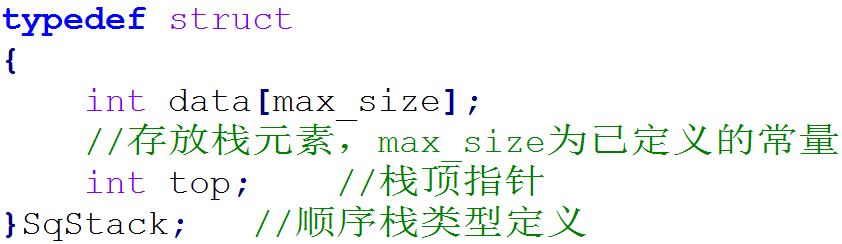
\includegraphics[width=2.81250in,height=0.81250in]{png-jpeg-pics/2808EF0D96046F76E3FF790F53B095F9.png}

考试中要用到栈的情况下,栈的声明以及操作可以写得很简单,下面给出实用的顺序栈的操作的写法:

{第一步:声明一个栈并初始化}

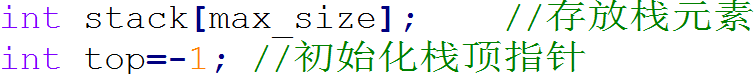
\includegraphics[width=2.39583in,height=0.23958in]{png-jpeg-pics/22CC74812EFCAA95829A01124BAA5E26.png}

{第二步:元素key入栈}

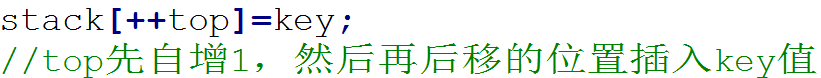
\includegraphics[width=2.62500in,height=0.25000in]{png-jpeg-pics/C052107CCE72649B9D5CC0ADBFEA8C17.png}

{第三步:出栈,值保存于变量key中}

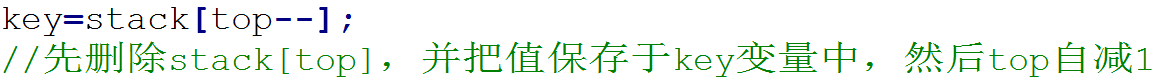
\includegraphics[width=3.33333in,height=0.23958in]{png-jpeg-pics/0800C6447573DC9A35298FF4895F511C.png}
